% https://tex.stackexchange.com/questions/45239/making-overlay-figures-in-tikz
\documentclass{standalone}
\usepackage{tikz}      
\usetikzlibrary{calc}  

\begin{document}
    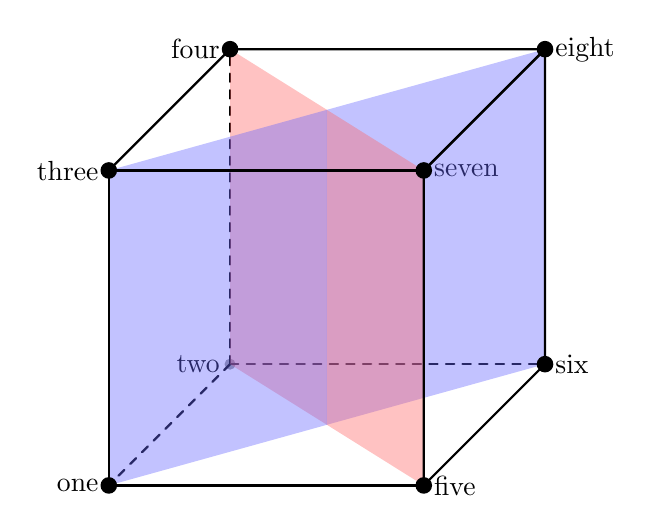
\begin{tikzpicture}[scale=4,fill opacity=0.4,thick,
                        line cap=round,line join=round]
    %% Define coordinate labels.
    % t(op) and b(ottom) layers
    \path \foreach \layer/\direction in {b/{0,0,0},t/{0,1,0}} {
        (\direction)
        \foreach \point/\label in {{0,0,0}/ll,{1,0,0}/lr,{1,0,-1}/ur,{0,0,-1}/ul} {
            +(\point) coordinate (\layer\label)
        }
        ($(\layer ll)!0.5!(\layer ur)$) coordinate (\layer md)
    };

    % Put text next to the labels as requested.
    % Funilly enough we need to set fill opacity to 1.
    \draw \foreach \text/\label/\anchor in {%
        one/bll/east,
        two/bul/east,
        three/tll/east,
        four/tul/east,
        five/blr/west,
        six/bur/west,
        seven/tlr/west,
        eight/tur/west} {
        (\label) node[anchor=\anchor,fill opacity=1] {\text}
    };

    % Draw left cube.
    \fill (0,0,-1) circle (0.5pt);
    \foreach \direction in {(0,0,1),(0,1,0),(1,0,0)} {
        \draw[dashed,black] (bul) -- + \direction;
    }
    \fill[blue!60] (bmd) -- (bur) -- (tur) -- (tmd);
    \fill[red!60]  (blr) -- (tlr) -- (tul) -- (bul);
    \fill[blue!60] (bll) -- (bmd) -- (tmd) -- (tll);
    \draw (bll) -- (blr) -- (tlr) -- (tll) -- cycle;
    \draw (blr) -- (bur) -- (tur) -- (tlr) -- cycle;
    \draw (tll) -- (tlr) -- (tur) -- (tul) -- cycle;
    \foreach \point in {bll,blr,bur,tll,tlr,tul,tur} {
        \fill[fill opacity=1] (\point) circle (0.75pt);
    }

    % Draw right cube.
    % \path (blr) + (0.65,0) coordinate (pos);
    % \foreach \direction in {(0,0,1),(0,1,0),(1,0,0)} {
    %     \draw[dashed] (pos) ++ (bul) -- + \direction;
    % }
    % \fill[blue!60] (pos) +(blr) -- +(bur) -- +(tur) -- +(tlr);
    % \fill[red!60]  (pos) +(bll) -- +(bul) -- +(tul) -- +(tll);
    % \draw (pos) +(tll) -- +(tlr) -- +(tur) -- +(tul) -- cycle
    %             +(tll) -- +(bll) -- +(blr) -- +(bur) -- +(tur)
    %             +(blr) -- +(tlr);
    \end{tikzpicture}
\end{document}